\chapter{Dynamical Systems Theory}
\label{DST}
\graphicspath{{chapter-8/Images/}}

\section{Introduction}
In the three-body problem, an important aspect is the invariant manifolds of the periodic orbits. An invariant manifold is a manifold embedded within a given phase space such that the manifold is invariant under the phase flow i.e. an orbit or solution that starts within an invariant manifold stays within this manifold \cite{nlde_book}. From an astrodynamics perspective, invariant manifolds are tube-like structures along which a spacecraft can travel without utilizing any energy \cite{moore2009_invariant}. The invariant manifold structures of libration points $L_1$ and $L_2$ are important for understanding the motion of a particle in a three-body problem that undergoes resonance hopping. Also of importance are the stable and unstable invariant manifolds associated with the periodic orbits around $L_1$ and $L_2$ since they are the phase space channels transporting material between the various realms within the three-body problem. It is the invariant manifold tubes that put limitations on the capture and escape properties of a third particle in motion in the three-body problem. Inside the invariant manifolds tubes, the motion of a particle consists of a set of paths called transit orbits and outside the manifolds, these transit orbits are not possible. The cylindrical tube like shaped unstable and stable manifolds associated with $L_1$ and $L_2$ are needed to understand the connections within the phase space \cite{invariant}. This chapter will provide a brief description on the underlying theory regarding dynamical systems and the invariant manifolds theory in the context of the three-body problem. The general discussion will be based on the (planar) circularly restricted three-body problem, but the concepts can easily be extended to higher fidelity models of the restricted three-body problem.

\section{(Planar) Circular Restricted Three-Body Problem}
We will consider the motion of a massless particle \textbf{P} which is being influenced by the gravitational attraction of two primary bodies with masses $m_1$ and $m_2$. These bodies are moving in a circular orbit around their barycentre or centre of mass. The particle \textbf{P} does not affect the motion of the two primary bodies. We define a certain mass parameter for this system as follows \cite{invariant}:
\begin{equation}
\label{massparam}
\mu = \frac{m_2}{m_1 + m_2}
\end{equation}
%
It is assumed that mass $m_1$ is larger than $m_2$. The two primary masses $m_1$ and $m_2$ are then rewritten in terms of this mass parameter as follows \cite{invariant}:
\begin{equation}
\begin{aligned}
\mu_1 &= 1 - \mu \\
\mu_2 &= \mu \\
\end{aligned}
\end{equation}
%
The geometry of the \gls{PCRTBP} is defined in a rotating frame where the origin of the frame is centered at the barycentre of the two primaries and the frame is rotating synchronously with the primary bodies' revolution rate around the barycentre. The geometry is depicted in \Cref{fig:rotframe} \cite{invariant}.
%
\begin{figure}[h]
\centering
\captionsetup{justification=centering}
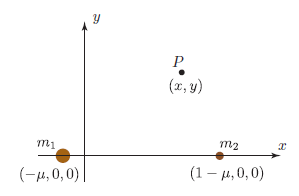
\includegraphics[scale=1]{rotframe.png}
\caption{Geometry of the \gls{PCRTBP} in rotating frame \cite{invariant}.}
\label{fig:rotframe}
\end{figure}
\FloatBarrier
%
The Hamiltonian equations of motion for the general circular restricted three-body problem (which can easily be converted to the \gls{PCRTBP} by making $z=\dot{z}=0$) in the rotating frame are given as follows \cite{invariant}:
\begin{equation}
\label{hamil_eom}
\begin{aligned}
\dot{x} &= p_x + y \\
\dot{y} &= p_y - x \\
\dot{z} &= p_z \\
\dot{p}_x &= p_y - x - U_x \\
\dot{p}_y &= -p_x - y - U_y \\
\dot{p}_z &= -U_z \\
\end{aligned}
\end{equation}
%
where $U$ is the gravitational potential and the subscripts denote against which term the partial derivative has been taken. The $p$ term are the momenta conjugate and are given as follows:
\begin{equation}
\begin{aligned}
p_x &= \dot{x} - y\\
p_y &= \dot{y}+x \\
p_z &= \dot{z}
\end{aligned}
\end{equation}
%
The corresponding energy integral of motion is also given as \cite{invariant}:
\begin{equation}
\label{energy_int}
E(x,y,z,\dot{x}, \dot{y}, \dot{z}) = \frac{1}{2}(\dot{x}^2 + \dot{y}^2 + \dot{z}^2) + U(x,y,z)
\end{equation}
%
This was a brief introduction to the (planar) circular restricted three-body problem. The equations of motion and energy integral of motion will be used in the following sections to understand the concepts of dynamical systems theory in astrodynamics.

\section{Energy Manifold, Hill's Region, and Zero Velocity Curves}
Considering the \gls{PCRTBP}, we have a four-dimensional phase space namely two position coordinates $x$, $y$ and two velocity coordinates $\dot{x}$ and $\dot{y}$. For a real value $e$, the equation $E_{kep} = e$ where $E_{kep}$ is called the Keplerian energy, denotes a three-dimensional set in the four-dimensional phase space. This three-dimensional set is termed the energy surface corresponding to the energy $e$ or simply an energy manifold \cite{invariant}.

Let $\mathcal{M}$ denote the energy manifold obtained by equating energy integral given by \Cref{energy_int} (take $z=\dot{z}=0$) to a constant real value $e$ \cite{invariant}:
\begin{equation}
\label{energy_manifold}
\mathcal{M}(\mu, e) = [(x,y,\dot{x},\dot{y})| E(x,y,\dot{x}, \dot{y}) = e]
\end{equation}
%
For a given value of $\mu$ and $e$, the energy manifold term $\mathcal{M}$ can be considered as a three-dimensional surface within the four-dimensional phase space. The projection of the energy manifold onto the $xy$ plane i.e. the position space of the rotating frame of reference, gives the region in which a particle with energy $e$ can undergo motion under the influence of the gravitational pull of the two primary masses $m_1$ and $m_2$. The regions of allowable motion are called \textit{Hill's Region}. This projection is given as follows \cite{invariant}:
\begin{equation}
\label{Hill}
M(\mu, e) = [(x,y) | U(x,y) \leq e]
\end{equation}
%
The boundary of the Hill region, $M(\mu,e)$, places bounds on the motion of the third particle and is called the zero velocity curve. The latter are a locus of points in the $xy$-plane where the kinetic energy of the particle vanishes i.e. the velocity is zero. The particle can have a non-zero velocity only on the side of this curve for which the particle has a positive kinetic energy. The other side of the curve is where the particle has negative energy and this is the region where motion is obviously not possible and is called the forbidden realm \cite{invariant}.

For a given mass parameter value, there are five basic configurations for the Hill's region each corresponding to the five intervals of the energy value $e$ in \Cref{energy_manifold}. Four of the cases are depicted in \Cref{fig:Hill}. The fifth case is not depicted here because it is graphically not relevant since in the fifth case, the particle is not subjected to any forbidden realm and can freely move about anywhere around the two primary bodies.
%
\begin{figure}[h]
\centering
\captionsetup{justification=centering}
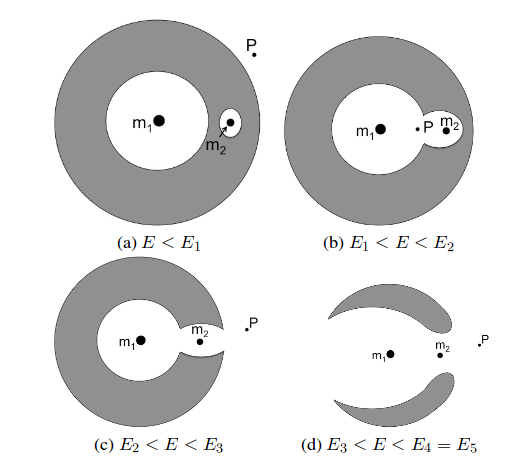
\includegraphics[scale=0.7]{hill_2.png}
\caption{Zero Velocity Curves for four cases of different energy values. The white regions in each case corresponds to the region accessible by the third particle for motion around the two primary masses. The shaded region are inaccessible by the particle and is called the forbidden realm. The outermost region beyond the shaded area, called exterior realm is accessible by particle. The fifth configuration, not shown here, is where the particle is not subjected to any forbidden realms and can freely move in the entire plane \cite{moore2009_invariant}.}
\label{fig:Hill}
\end{figure}
\FloatBarrier
%
We will discuss the five cases of energy values now and how they affect the motion of the particle in the \gls{PCRTBP} \cite{invariant}:
\begin{itemize}
\item $E<E_1$: If the energy of the particle is less than the critical value $E_1$ then the particle cannot move from the accessible realm around $m_1$ to the accessible realm around $m_2$ and vice-a-versa.
\item $E_1<E<E_2$: For the particle energy just above the critical energy $E_1$, a small opening or a "neck" forms between the accessible realms of $m_1$ and $m_2$ from the previous case. The $L_1$ point is in this neck opening.  The particle can thus move through this neck and this transport is controlled by the invariant manifold associated with the $L_1$ point.
\item $E_2<E<E_3$: If the energy of the particle is just above the critical value $E_2$ then another neck opens up connecting the realm around $m_2$ to the exterior realm. This neck also corresponds to the $L_2$ point. The particle can now move between the internal realms around the primary masses and also to the exterior realm through the two necks as seen in case 3 in \Cref{fig:Hill}.
\item $E_3<E<E_4=E_5$: The particle in this energy range results in opening up the neck region between the $m_1$ realm and the exterior realm and this neck region corresponds to the $L_3$ libration point.
\item $E_4=E_5 < E$: For particle in this energy interval, the forbidden realm vanishes and the particle can move everywhere in the position space.
\end{itemize}
%
Each critical value of energy as discussed above, $E_i$, $i=1...4$ corresponds to the corresponding libration points $L_i$, $i=1...4$ \cite{invariant}. In the next section we will look at how the libration points are obtained for a given system.

\section{Libration Points}
We will still consider the \gls{PCRTBP}. The equations of motion for this problem are given as:
\begin{equation}
\label{planareom}
\begin{aligned}
\dot{x} &= v_x \\
\dot{y} &= v_y \\
\dot{v}_x &= 2v_y - U_x \\
\dot{v}_y &= -2v_x - U_y
\end{aligned}
\end{equation}
%
To find the libration points, the right-hand sides of each expression in \Cref{planareom} is set to zero. In doing so we get two equations which have to solved to obtain the equilibrium points namely $U_x = 0$ and $U_y = 0$. The libration points are also called equilibrium points and the equilibria in the four-dimensional phase space is of the form $(x_e,y_e,0,0)$ where the critical points of the potential function are given as $(x_e,y_e)$. In the \gls{PCRTBP} there are 5 equilibrium or libration points out of which the first three, $L_1$ , $L_2$, and $L_3$ lie on the $x$-axis and are collinear. $L_4$ and $L_5$ are not collinear and are located in the $xy$-plane such that $y\neq0$. A few definitions might come handy. Assume $r_1$ is the distance from the primary $m_1$ to the third particle and similarly $r_2$ is the distance from the primary $m_2$ to the particle. These terms are obtained as follows \cite{invariant}:
\begin{equation}
\label{r1r2}
\begin{aligned}
r_1^2 &= (x+\mu_2)^2 + y^2 + z^2 \\
r_2^2 &= (x - \mu_1)^2 + y^2 + z^2
\end{aligned}
\end{equation}
%
Of course for the planar problem the $z$-term in \Cref{r1r2} would become 0. The potential term is given as \cite{invariant}:
\begin{equation}
\label{planarpot}
\begin{aligned}
U(x,y) &= -\frac{1}{2}(x^2 + y^2) - \frac{\mu_1}{r_1} - \frac{\mu_2}{r_2} - \frac{1}{2}\mu_1  \mu_2\\
&= -\frac{1}{2}(\mu_1 r_1^2 + \mu_2 r_2^2) - \frac{\mu_1}{r_1} - \frac{\mu_2}{r_2}
\end{aligned}
\end{equation}
%
We will start with the process to obtain the non-collinear libration points. After rearranging terms in \Cref{r1r2} the following expression is obtained \cite{invariant}:
\begin{equation}
x^2 + y^2 = (1-\mu)r_1^2 + \mu r_2^2 - \mu (1-\mu)
\end{equation}
%
Substituting this into \Cref{planarpot} we get:
\begin{equation}
-U(r_1, r_2) = \frac{1}{2}(1-\mu)r_1^2 + \frac{1}{2}\mu r_2^2 + \frac{1-\mu}{r_1} + \frac{\mu}{r_2}
\end{equation}
%
The partial derivatives of $U$ equated to 0 will give the libration points 4 and 5:
\begin{equation}
\begin{aligned}
U_x &= U_{r_1} \frac{\partial r_1}{\partial x} + U_{r_2} \frac{\partial r_2}{\partial x} = 0 \\
U_y &= U_{r_1} \frac{\partial r_1}{\partial y} + U_{r_2} \frac{\partial r_2}{\partial y} = 0
\end{aligned}
\end{equation}
%
solving which leads to:
\begin{equation}
\begin{aligned}
0 &= -U_{r_1} = \mu r_2 - \frac{\mu}{r_2^2} \\
0 &= -U_{r_2} = (1-\mu) r_1 - \frac{1-\mu}{r_2^2}
\end{aligned}
\end{equation}
%
Solving which we get the unique solution $r_1=r_2=1$ meaning that the $L_4$ and $L_5$ libration points lie at equal distances from the two primary masses. $L_4$ lies in the positive $y$ segment and $L_5$ lies in the negative. Now we will calculate the collinear equilibrium points. In this case $y=0$ and so the potential function would be rewritten as \cite{invariant}:
\begin{equation}
\label{pot_coll}
U(x,0) = -\frac{1}{2}x^2 - \frac{1-\mu}{|x+\mu|} - \frac{\mu}{|x - 1 + \mu|}
\end{equation}
%
We have three intervals along the $x$-axis as can be seen in \Cref{fig:rotframe} namely $(-\infty, -\mu )$, $(-\mu, 1-\mu )$, and $(1- \mu , \infty)$. Note that these intervals are only for the $x$-coordinate and the second term in each bracket does not correspond to the $y$-coordinate. For all these intervals, the potential function tends to $-\infty$. Also, the second partial derivative of the potential function from \Cref{pot_coll} is always negative meaning that the potential function is concave in all three intervals. Thus each interval has precisely one critical point. These points are the three remaining libration points. Calculating the $x$ coordinate of the collinear libration points requires us to finding the maximum (due to concaveness) of the potential function. The distance from $L_1$ and $L_2$ to the mass $m_2$ is given by the following equation \cite{invariant}:
\begin{equation}
\label{gammadist}
\gamma^5 \mp (3 - \mu)\gamma^4 + (3-2\mu)\gamma^3 - \mu \gamma^2 \pm 2 \mu \gamma - \mu = 0
\end{equation}
%
A similar equation can be found for the distance of $L_3$ to the mass $m_1$. The solution to the distance equation is obtained by using a series expansion method and are given as \cite{invariant}:
\begin{equation}
\begin{aligned}
\gamma_1 &= r_h (1- \frac{1}{3}r_h - \frac{1}{9}r_h^2+...) \\
\gamma_2 &= r_h (1 + \frac{1}{3}r_h - \frac{1}{9}r_h^2+...)
\end{aligned}
\end{equation}
%
where $r_h$ is called the Hill radius and is defined by the equation $r_h = \frac{\mu}{3}^{1/3}$. Using the Newton-Raphson method and taking the Hill radius as initial value, the solutions $\gamma_1$ and $\gamma_2$ to \Cref{gammadist} can be found. This is how the libration points can be found in the case of the \gls{PCRTBP} and a similar approach can be applied for higher-fidelity models.

\section{Invariant Manifolds of a Periodic Orbit}
To compute the invariant manifolds of a periodic orbit, one needs two mathematical tools namely the monodromy matrix and the Poincar\'e maps. These tools will also be helpful in assessing the stability of periodic orbits.

\subsection{Monodromy Matrix}
We will consider an autonomous equation of the form $\dot{x} = f(x)$ with $x(0) = x_0$. The periodic solution for this is given as $x(t)$ with a period of $T$. Now a trajectory, or solution, that starts at a perturbed initial state vector i.e. $x_0 + \delta x_0$ will after one full period experience a displacement by \cite{invariant}:
\begin{equation}
\delta x(T) = \phi(T;x_0 + \delta x_0) - \phi(T; x_0)
\end{equation}
%
which in first order is written as:
\begin{equation}
\delta x(T) = \phi(T) \delta x_0
\end{equation}
%
where $\phi(T)$ is the state transition matrix for one time period T. This is the monodromy matrix which determines whether a perturbation in the initial state vector tends to grow or decay, and is defined as \cite{invariant}:
\begin{equation}
M \equiv \phi(T) = \frac{\partial \phi(T;x_0)}{\partial x_0}
\end{equation}
%
Some important mathematical properties relating to the monodromy matrix which will be helpful are stated as follows \cite{invariant}:
\begin{itemize}
\item Floquet Theorem: $\phi(t) = P(t) e^{Rt}$ where P(t) is periodic with a period of T and R is a constant matrix
\item $\phi(kT) = M^k$
\item M has an eigenvalue equal to 1 with an eigenvector that is tangent to the periodic orbit at $x_0$ and this eigenvector is given as $\dot{x}(0) = f(x_0)$
\end{itemize}
%
The eigenvalues $\lambda$ of the monodromy matrix are called Floquet or characteristic multipliers and each number $\sigma$ related to eigenvalue as $\lambda = e^{\sigma T}$ is called the Floquet or characteristic exponent. These terms are used for studying the local stability of a periodic solution.

\subsection{Poincar\'e Maps}
These maps are useful to study the flow near a periodic orbit. Let's define a co-dimension 1 surface of section as $\sum$ such that all trajectories that cross it in a neighborhood of $q\in \sum$ satisfy two requirements namely: the trajectories intersect the surface of section transversely and that they cross the surface in the same direction \cite{invariant}. If $T_{\sum}(q)$, where $q\in \sum$, is the time taken for a trajectory $\phi (t;q)$ to return to $\sum$ for the first time, then the Poincar\'e map is given as \cite{invariant}:
\begin{equation}
P(q) \equiv \phi (T_{\sum} (q); q)
\end{equation}
%
So in plain words, a Poincar\'e map is created by allowing trajectories to intersect with the Poincar\'e section. This is shown pictorially in \Cref{fig:map}.
%
\begin{figure}[h]
\centering
\captionsetup{justification=centering}
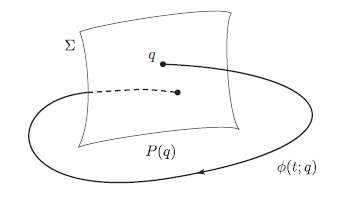
\includegraphics[scale=0.7]{map.png}
\caption{Poincar\'e map generated by trajectories intersecting the Poincar\'e section \cite{invariant}.}
\label{fig:map}
\end{figure}
\FloatBarrier
%
A periodic trajectory would then be the one which intersects the section at the same fixed point $q$ where $q = \phi(T;q)$. The stability of a periodic orbit is obtained by checking whether the point $q$ is an attractor or repellor in the map. To do this we linearize the Poincar\'e map around the fixed point $q$ as follows \cite{invariant}:
\begin{equation}
\frac{\partial P(q)}{\partial q} = \frac{\partial \phi (T;q)}{\partial q}
\end{equation}
%
The eigenvalues of this linearization are then calculated and if the moduli of all eigenvalues is smaller than 1 then the point $q$ is stable and if the modulus of any one eigenvalue is larger than 1 then $q$ is unstable. Similarly in case of the monodromy matrix $M$, apart from the one eigenvalue which is equal to one, if the modulus of all remaining eigenvalues of $M$ is less than one then the periodic orbit is stable otherwise even if the modulus of one of the eigenvalue is greater than one then the orbit is unstable.

\subsection{Computation of Invariant Manifolds}
Given the monodromy matrix $M = \phi(T)$, its eigenvalues are first calculated. The eigenvectors associated with the modulus of eigenvalues greater than 1 are in the unstable direction whereas the eigenvectors associated with modulus of eigenvalues less than 1 are in the stable direction. Let $Y^s (X_0)$ denote the normalized stable eigenvector and $Y^u (X_0)$ denote the normalized unstable eigenvector. These are used to get the approximate manifolds as \cite{invariant}:
\begin{equation}
\begin{aligned}
X^s (X_0) &= X_0 + \epsilon Y^s (X_0) \\
X^u (X_0) &= X_0 + \epsilon Y^u (X_0)
\end{aligned}
\end{equation}
%
where $X^s$ and $X^u$ are the initial guesses for the stable and unstable manifolds respectively at $X_0$ along the periodic orbit. The term $\epsilon$ denotes a small displacement from $X_0$. By numerically integrating the unstable eigenvector forward in time using both $\pm \epsilon$ we can generate trajectories shadowing the two branches of the unstable manifold and in a similar way, by integrating the stable eigenvector backwards in time we can generate trajectories shadowing the two branches of the stable manifold. So this is how the invariant manifold for the periodic orbit are obtained \cite{invariant}.

\section{Conclusion}
This was a brief chapter describing various elements that are utilized when it comes to applying the dynamical systems theory to astrodynamics problems. Many books have been written in this regard and for some readers this chapter might seem obscure but the purpose of including it in this literature study report was to understand the basics of dynamical systems theory and its application to celestial mechanics.
